\chapter{Superposition}
\section{Principles}
\begin{definition}{Principle of superposition}{posoup}
	When 2 or more waves \it{of the same kind} overlap, the resultant displacement
	at any point equals the \it{vector sum} of the \it{individual displacements}
	at that point.
\end{definition}

\begin{definition}{Interference}{interference}
	The phenomenon where 2 or more waves superpose to form a resultant wave,
	whose amplitude is given by the Principle of Superposition.
\end{definition}

\begin{definition}{Coherence}{coherent}
	Coherent wave sources are those who maintain a \it{constant phase difference}
	between them.
\end{definition}

An interference pattern is \bf{observable} iff
\begin{enumerate}
	\item sources are \it{coherent}
	\item waves are approximately the same amplitude
	\item transverse waves are unpolarised or share the same polarisation direction
\end{enumerate}

\bf{Constructive interference} when two waves meet \it{in phase} \(\implies\) maximum resultant amplitude, maximum intensity.
\bf{Destructive interference} when two waves meet \it{in anti-phase} \(\implies\) minimum resultant amplitude, minimum intensity.

For two waves of the same amplitude \(A\),
\begin{table}[htpb]
	\centering
	\begin{tabular}{r c c}
		\toprule
		\hil{\bf{sources in phase}}                  & constructive                 & destructive                  \\
		\midrule
		amplitude \(A_\text{res}\)                   & \(2A\)                       & \(0\)                        \\
		intensity \(I_\text{res}\)                   & max                          & min                          \\
		path diff.~\(\delta\)                        & \(n\lambda\)                 & \(\f{1}{2}\ab(2n+1)\lambda\) \\
		phase diff.~\(\Delta\phi\)                   & \(2k\pi\)                    & \(\ab(2k+1)\pi\)             \\
		\toprule
		\hil[jiyoyellow]{\bf{sources in anti-phase}} & constructive                 & destructive                  \\
		\midrule
		amplitude \(A_\text{res}\)                   & \(0\)                        & \(2A\)                       \\
		intensity \(I_\text{res}\)                   & min                          & max                          \\
		path diff.~\(\delta\)                        & \(\f{1}{2}\ab(2n+1)\lambda\) & \(n\lambda\)                 \\
		phase diff.~\(\Delta\phi\)                   & \(\ab(2k+1)\pi\)             & \(2k\pi\)                    \\
		\bottomrule
	\end{tabular}
	\caption{Constructive and destructive interference}
	\label{tab:interference-types}
\end{table}

\section{Double slit}
For a double slit with distance between slits \(d\), distance
of slits to screen \(L\) and incident light of wavelength \(\lambda\).
\begin{figure}[htpb]
	\centering
	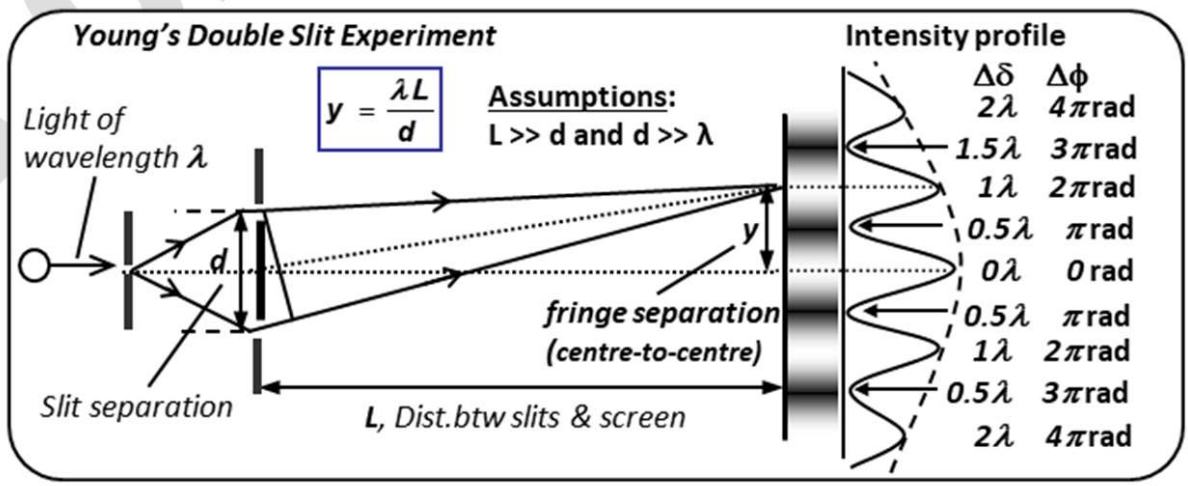
\includegraphics[width=\textwidth]{assets/double-slit.png}
	\caption{Double slit}
	\label{fig:double-slit}
\end{figure}

\it{Where can we find maxima/minima?} At angles \(\theta\), where
\begin{itemize}
	\item maxima (constructive): \(d\sin\theta=m\lambda\), where \(m \in \integers_0\)
	\item minima (destructive): \(d\sin\theta=(m-\num{0.5})\lambda\), where \(m \in \integers\)
\end{itemize}

Slits are separated by a \bf{slit separation} \(\Delta y\) where
\[\Delta y=\f{\lambda L}{d}\]

The assumption is that \(L\gg d\) and \(d \gg \lambda\).

\section{Diffraction grating}
For a diffraction grating with \(\lf{1}{d}\) slits per unit length (\(d\) is the slit spacing),
and incident light of wavelength \(\lambda\),
\[d\sin\theta=n\lambda\]
where \(n\) is the order.
\begin{figure}[htpb]
	\centering
	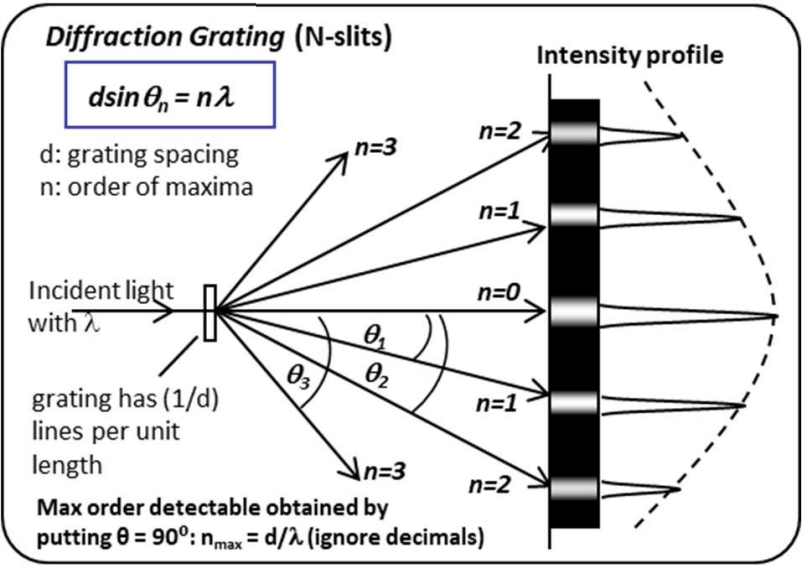
\includegraphics[width=0.75\textwidth]{assets/diffraction-grating.png}
	\caption{Diffraction grating}
	\label{fig:diffraction-grating}
\end{figure}


\section{Single slit diffraction}
\begin{marginfigure}
	\centering
	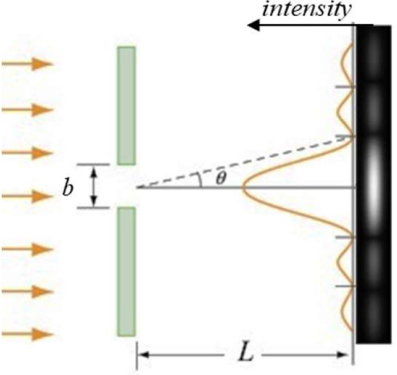
\includegraphics[width=\textwidth]{assets/single-slit.png}
	\caption{Single slit}
	\label{fig:single-slit}
\end{marginfigure}
With a single slit of width \(b\) and incident light of wavelength \(\lambda\),
the \bf{first minimum intensity} is at \(\theta\) where
\[\sin\theta=\f{\lambda}{b}\]

\begin{definition}{Rayleigh criterion}{rayleigh}
	Two images are \it{just resolvable} when the centre of one image's
	diffraction pattern is \it{directly over} the first minimum of the other's diffraction pattern.
\end{definition}
\begin{marginfigure}
	\centering
	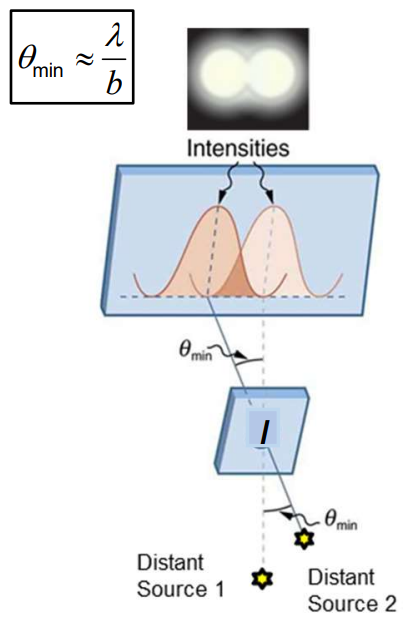
\includegraphics[width=.8\textwidth]{assets/rayleigh.png}
	\caption{Rayleigh criterion}
	\label{fig:rayleigh}
\end{marginfigure}
The aperture's \bf{resolving power} is then
\[\theta_{\min} \approx \f{\lambda}{b}\]

\section{Stationary waves}
\begin{marginfigure}
	\centering
	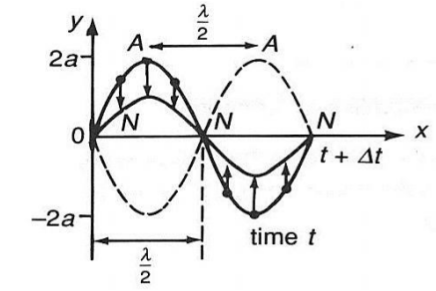
\includegraphics[width=\textwidth]{assets/stationary-wave.png}
	\caption{Stationary wave \(y\) versus \(x\)}
	\label{fig:stationary-waves}
\end{marginfigure}
\begin{definition}{Stationary waves}{stationary-waves}
	are formed when two similar waves of the \it{same frequency},
	\it{same speed}, and \it{same amplitude} \(A\) travel in
	\it{opposite directions} and superpose.
\end{definition}
\begin{itemize}
	\item \bf{Antinodes} are where amplitude is a maximum (\(2A\));
	      \bf{nodes} are where amplitude is a minimum (\num{0}).
	\item Particles in the same segment are in phase; particles in adjacent segments are in antiphase.
	\item Wavelength \(\lambda = 2\cdot\text{distance from A to A}\)
	\item Energy is not propagated.
\end{itemize}

\subsection{String fixed at two ends}
Where \(L\) is the string's length, the frequency and wavelength at the \(n\)th harmonic are
\begin{align*}
	f_n       & = n\f{v}{2L} \\
	\lambda_n & = \f{2L}{n}
\end{align*}

\subsection{Air columns}
Air columns come in closed pipes and open pipes.
\begin{table}[htpb]
	\centering
	\begin{tabular}{r l l}
		\toprule
		               & closed pipe                                      & open pipe                \\
		\midrule
		disp.~A/N      & disp.~N at closed end, disp.~A at open end       & both ends disp.~A        \\
		pressure A/N   & pressure A at closed end, pressure N at open end & both ends pressure N     \\
		\(f_n\)        & \(\lf{nv}{4L},\:n=2k+1\)                         & \(\lf{nv}{2L}\)          \\
		\(\lambda_n\)  & \(\lf{4L}{n},\:n=2k+1\)                          & \(\lf{2L}{n}\)           \\
		end correction & \(\lf{\lambda}{4}=L+c\)                          & \(\lf{\lambda}{2}=L+2c\) \\
		\bottomrule
	\end{tabular}
	\label{tab:closed-open-pipes}
	\caption{Closed and open pipes}
\end{table}
